\documentclass[border=10pt]{standalone}

\usepackage{xcolor}

\definecolor{miamired}{RGB}{200,16,46}
\definecolor{darkgreen}{rgb}{0.09, 0.45, 0.27}
\definecolor{links}{HTML}{2A1B81}

\usepackage[export]{adjustbox}
\usepackage{amsfonts}
\usepackage{amsmath}
\usepackage{amssymb}
\usepackage{animate}
\usepackage{array}
\newcolumntype{M}[1]{>{\arraybackslash\hspace{0pt}}p{#1}}
\usepackage[justification=centering]{caption}
\usepackage{colortbl}
\usepackage{etoolbox}
\usepackage{fancybox}
\usepackage{forest}
\usepackage{framed}
\usepackage{graphics}
\usepackage{graphicx}
\graphicspath{ {Figures/} }
\usepackage{hyperref} 
\usepackage[utf8]{inputenc}
\usepackage{makecell}
\usepackage{mathtools}
\usepackage{marvosym}
\usepackage[framemethod=default]{mdframed}
%\addmediapath{ {Figures/} }
\usepackage{multicol}
%\usepackage{multimedia}
\usepackage{multirow}
\usepackage{pgfplots} %for tikzpictures
\pgfplotsset{compat=1.18}
\usepackage{sidecap}
\usepackage{smartdiagram}
\usepackage{soul}
\usepackage{subfigure}
\usepackage{tikz}
\usetikzlibrary{shapes.geometric, arrows}
\usepackage{times}
\urlstyle{same}
\usepackage{wasysym} % for smiley faces
\usepackage{wrapfig}



\begin{document}
	
	
	\centering
		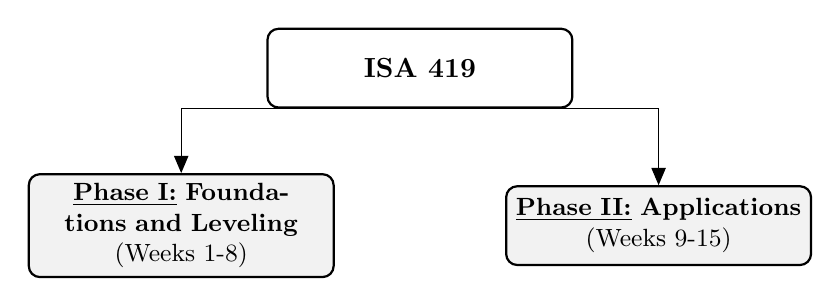
\begin{tikzpicture}[node distance=2cm, font=\small]
			\tikzstyle{start} = [rectangle, rounded corners, minimum width=0.3\textwidth, minimum height=1cm,text badly centered, text width=0.3\textwidth, draw=black, thick,font=\normalfont]
			
			\tikzstyle{categories} = [rectangle, rounded corners, minimum width=0.3\textwidth, minimum height=1cm,text centered, text width=0.3\textwidth, draw=black, fill=gray!10, thick]
			
			
			\tikzstyle{arrow} = [->,>= triangle 45]
			
			% Begining of the creation of the figure
			\node (start) [start] {\textbf{ISA 419}};
			
  		% Level 1 nodes
  		\node (ba) [categories, below of = start, xshift=-0.25\textwidth] {\textbf{\underline{Phase I:} Foundations and Leveling} \\ (Weeks 1-8)};
  		\node (app) [categories, below of = start, xshift = 0.25\textwidth] {\textbf{\underline{Phase II:} Applications} \\ (Weeks 9-15)};	
  		
  		% Arrows
  		\draw [arrow] (start.south) -| (ba);
  		\draw [arrow] (start.south) -| (app);
		\end{tikzpicture}
	
	
\end{document}


